\chapter{Implementacija i korisničko sučelje}
		
		
		\section{Korištene tehnologije i alati}
		
			\indent \indent Komunikacija grupe se odvijala putem aplikacije \href{https://www.whatsapp.com/}{WhatsApp\footnote{https://www.whatsapp.com/}}, dok je za održavanje sastanaka na daljinu korištena aplikacija \href{https://www.microsoft.com/en-us/microsoft-teams/group-chat-software/}{MicrosoftTeams\footnote{https://www.microsoft.com/en-us/microsoft-teams/group-chat-software/}}, koja pruža opciju video poziva. Sustav \href{https://git-scm.com/}{Git\footnote{https://git-scm.com/}} je omogućio upravljanje različitim verzijama programskog koda i dokumentacije uz udaljeni repozitorij na web platformi \href{https://github.com/}{GitHub\footnote{https://github.com/}}. Dokumentacija je pisana u programskom jeziku \href{https://www.latex-project.org/}{LaTeX\footnote{https://www.latex-project.org/}}, a za izradu UML dijagrama korišteni su alati \href{https://erdplus.com/}{ERDPlus\footnote{https://erdplus.com/}} i \href{https://astah.net/products/astah-uml/}{Astah UML\footnote{https://astah.net/products/astah-uml/}} sa studentskom licencom.
				
			\indent Korištena je kombinacija razvojnih okruženja ovisno o developeru. Aplikacija je napisana koristeći \href{https://eclipseide.org/}{Eclipse IDE\footnote{https://eclipseide.org/}} i \href{https://www.jetbrains.com/idea/}{IntelliJ IDEA\footnote{https://www.jetbrains.com/idea/}}, dok je za pisanje dokumentacije korišteno razvojno okruženje \href{https://code.visualstudio.com/}{Visual Studio Code\footnote{https://code.visualstudio.com/}}. Eclipse je \textit{open-source} integrirano razvojno okruženje koje se dominantno koristi za razvoj Java aplikacija uz Java razvojne alate. Moguće je prilagoditi okruženje za razvoj web-stranica, web-aplikacija i mobilnih aplikacija uz alate za razvoj programskih aplikacija. Intellij IDEA je integrirano razvojno okruženje tvrtke JetBrains za razvoj računalnih programa u Javi, Kotlinu te drugim programskim jezicima koji se oslanjaju na Java virtualni stroj. Sadrži brojne značajke koje znatno olakšavaju pisanje aplikacija kao što su posebni alati za radne okvire Spring i Spring Boot, pametno popunjavanje koda i podrška pri radu s HTTP porukama. Visual Studio Code je integrirano razvojno okruženje tvrtke Microsoft koje se koristi za razvoj računalnih programa u brojnim računalnim jezicima poput Python, C/C++ i Java. Sva korištena razvojna okruženja su podržana na operacijskim sustavima Microsoft, Linux i macOS. \\
				
			\indent Aplikacija je napravljena u radnom okviru \href{https://spring.io/projects/spring-boot/}{Spring Boot\footnote{https://spring.io/projects/spring-boot/}} kao \href{https://maven.apache.org/}{Maven\footnote{https://maven.apache.org/}} projekt. Za izradu \textit{backenda} aplikacije korišten je programski jezik \href{https://www.java.com/en/}{Java\footnote{https://www.java.com/en/}}, a za izradu \textit{frontenda} je korišten \href{https://react.dev/}{React\footnote{https://react.dev/}} i programski jezik \href{https://www.javascript.com/}{JavaScript\footnote{https://www.javascript.com/}}. Spring Boot je specijalizacija radnog okvira Spring koji se temelji na višeslojnoj arhitekturi čiji je cilj ubrzati i pojednostaviti razvoj web-aplikacija. Spring boot pruža podršku za automatsko definiranje programskih zahtjeva prilikom stvaranja projekata, za ugrađeni server Tomcat i za bazu podataka. Maven je programska podrška za organizaciju projekata i automatizaciju pokretanja aplikacija. Koristimo \textit{in-memory} \href{https://www.h2database.com/html/main.html}{H2\footnote{https://www.h2database.com/html/main.html}} bazu podataka koju pruža Spring Boot. React je biblioteka u JavaScriptu za izgradnju korisničkih sučelja temeljenih na komponentama koju održava Facebook. Glavne značajke React-a su ponovno korištenje web komponenti i ponovno prikazivanje samo komponente koje su promijenjene, a ne cijelu stranicu. Uspostava sobe za video poziv je omogućena preko \href{https://www.daily.co/}{Daily\footnote{https://www.daily.co/}} WebRTC usluga. Ispitivanje projekta je provedeno pomoću \href{https://www.selenium.dev/documentation/webdriver/}{Selenium WebDriver\footnote{https://www.selenium.dev/documentation/webdriver/}}.

		\eject 
		
	
		\section{Ispitivanje programskog rješenja}
			
			%\textbf{\textit{dio 2. revizije}}\\
			
			 %\textit{U ovom poglavlju je potrebno opisati provedbu ispitivanja implementiranih funkcionalnosti na razini komponenti i na razini cijelog sustava s prikazom odabranih ispitnih slučajeva. Studenti trebaju ispitati temeljnu funkcionalnost i rubne uvjete.}
	
			
			\subsection{Ispitivanje komponenti}
			%\textit{Potrebno je provesti ispitivanje jedinica (engl. unit testing) nad razredima koji implementiraju temeljne funkcionalnosti. Razraditi \textbf{minimalno 6 ispitnih slučajeva} u kojima će se ispitati redovni slučajevi, rubni uvjeti te izazivanje pogreške (engl. exception throwing). Poželjno je stvoriti i ispitni slučaj koji koristi funkcionalnosti koje nisu implementirane. Potrebno je priložiti izvorni kôd svih ispitnih slučajeva te prikaz rezultata izvođenja ispita u razvojnom okruženju (prolaz/pad ispita). }
			Ispitivanje jedinica provedeno je uz pomoć okvira za ispitivanje \href{https://junit.org/junit5/}{JUnit 5}\footnote{\url{https://junit.org/junit5/}}. Provedeno je ispitivanje za važne elemente klasa SearchService, PersonService, Recipe i StarRating te sučelja PersonRepository. Rezultat pokretanja testova prikazan je na slici, a sami testovi opisani su u nastavku.
			\begin{figure}[H]
				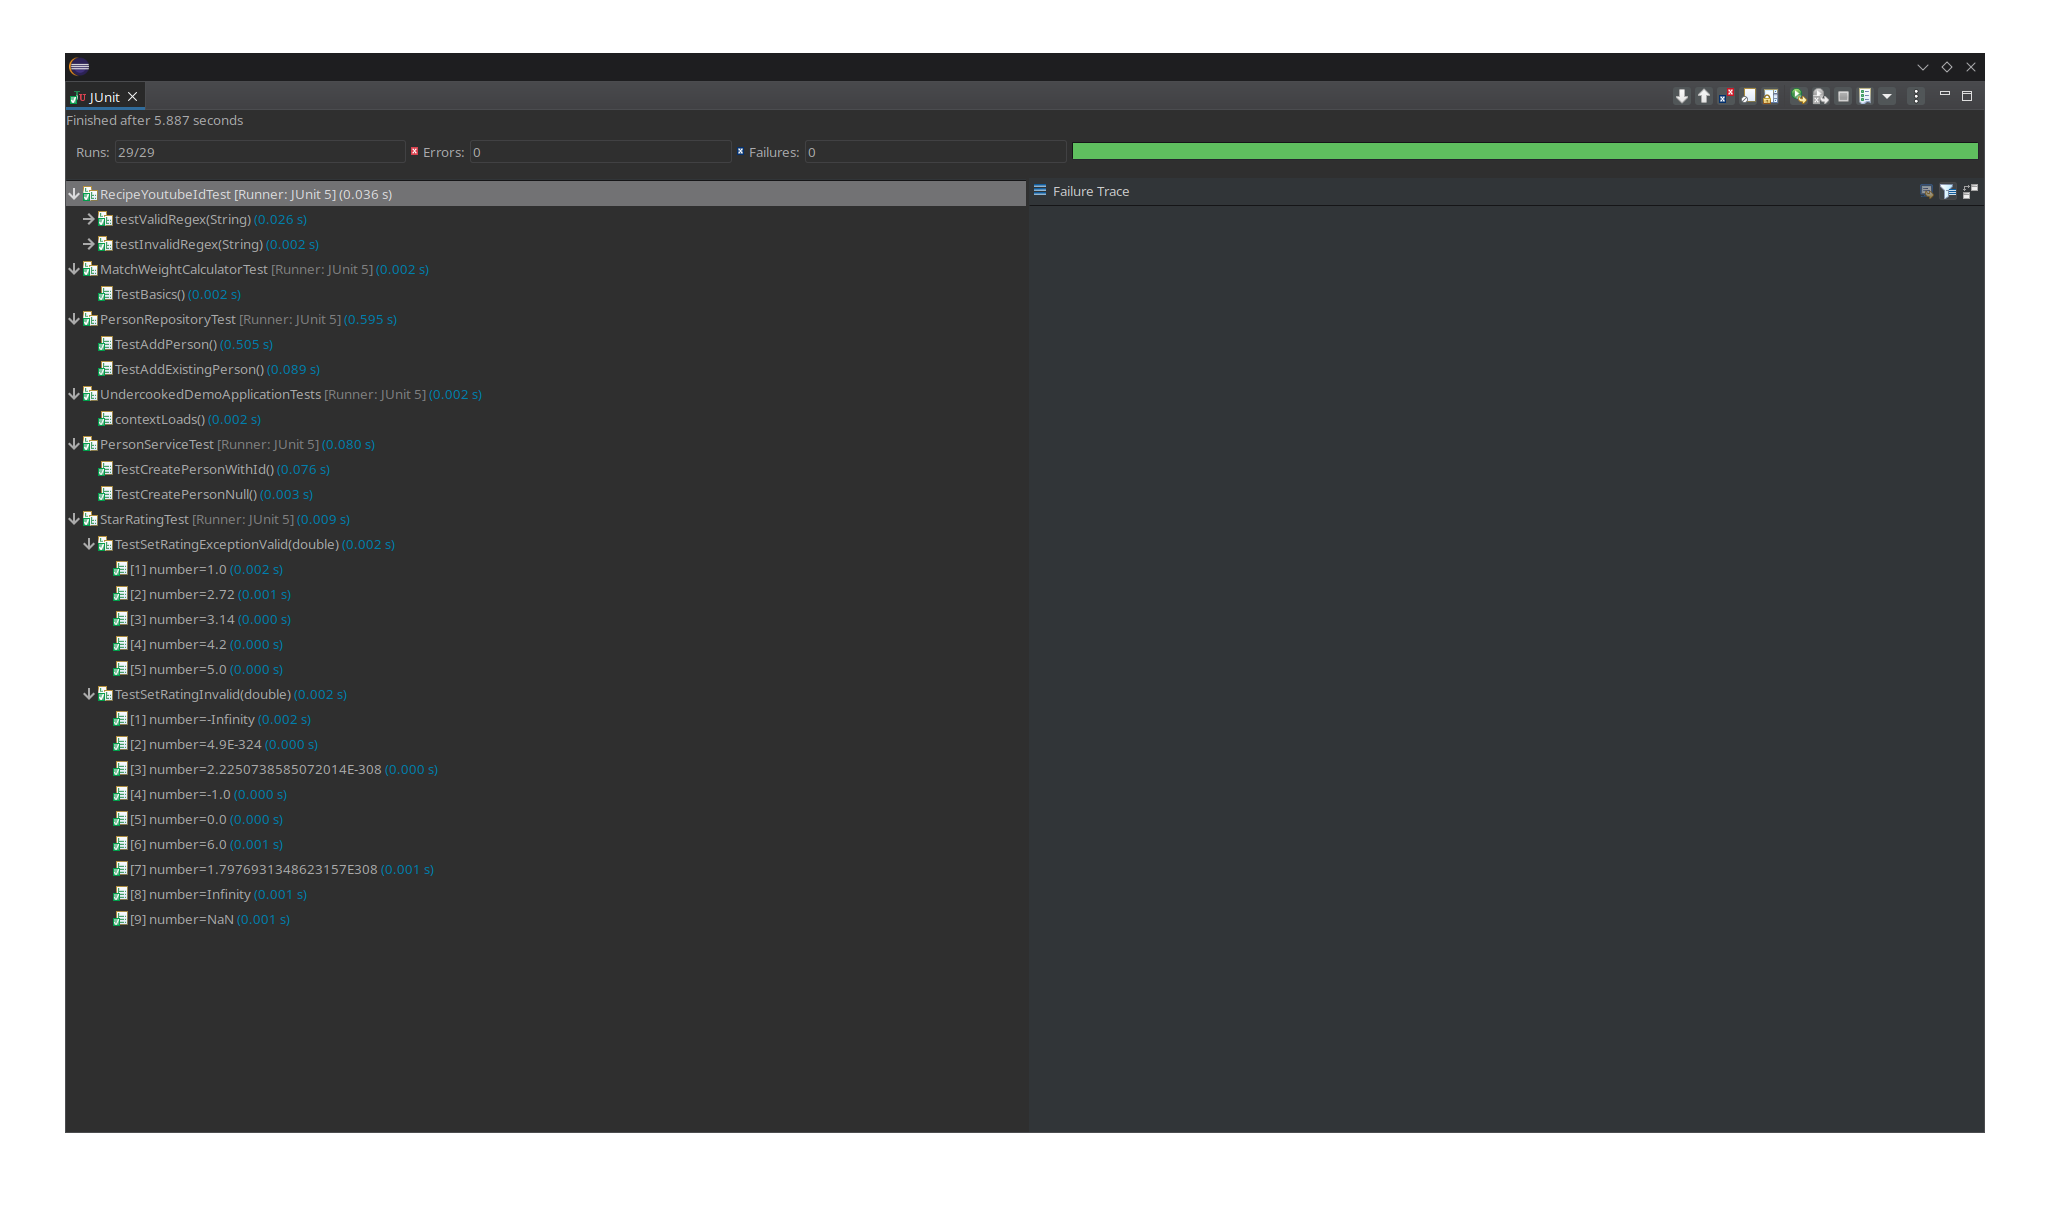
\includegraphics[scale=0.3]{slike/unit_test_screenshot.png} %veličina slike u odnosu na originalnu datoteku i pozicija slike
				\centering
				\caption{Rezultati unit testova}
				\label{fig:Rezultati unit testova}
			\end{figure}
			
			\noindent\textbf{Ispitivanje klase SearchService}
			
			Klasa SearchService omogućava pretraživanje recepata prema ključnim riječima naslova i opisa. Za ispravan rad pretraživanja važna je ugniježđena klasa MatchWeightCalculator koja računa sličnost između argumenata pretrage i rezultata. Metoda pow kao parametar uzima decimalni broj i vraća decimalni broj koji asimptotski raste prema dva za veću vrijednost parametra.
			\begin{lstlisting}
public class MatchWeightCalculatorTest {
	@Test
	public void TestBasics() {
		Assert.isTrue(SearchService.MatchWeightCalculator.pow(0) == 0, ""); // Nula u nuli,
		Assert.isTrue(SearchService.MatchWeightCalculator.pow(1) == 1, ""); // jedan u jedan,
		Assert.isTrue(SearchService.MatchWeightCalculator.pow(2) == 1.5, ""); // raste
		Assert.isTrue(SearchService.MatchWeightCalculator.pow(3) == 1.75, ""); // i raste
		Assert.isTrue(SearchService.MatchWeightCalculator.pow(Double.POSITIVE_INFINITY) == 2, ""); // asimptotski prema dva.
	}
}
			\end{lstlisting}
			
			\noindent\textbf{Ispitivanje klase PersonService}
			
			Klasa PersonService služi za upravljanje podatcima vezanim uz korisnike stranice. Ispitano je kako se sustav ponaša pri neispravnom dodavanje osobe u bazu podataka.
			\begin{lstlisting}
@SpringBootTest
@AutoConfigureTestDatabase(connection = EmbeddedDatabaseConnection.H2)
public class PersonServiceTest {
	
	@Autowired
	PersonService personService;
	
	@Test
	public void TestCreatePersonNull() {
		Person person = null;
		String expected = "Person object must be given";
		
		Exception e = assertThrows(IllegalArgumentException.class,
		() -> personService.createPerson(person));
		assertEquals(expected, e.getMessage());
	}
	
	@Test
	public void TestCreatePersonWithId() {
		Person person = new Person();
		person.setUsername("RMS");
		person.setEmail("rms@gnu.org");
		person.setName("Richard");
		person.setSurname("Stallman");
		person.setPassword(new BCryptPasswordEncoder().encode("superSecretPassword123"));
		person.setAdmin(false);
		person.setId((long) 1337);
		String expected = "Person ID must be null, not: 1337";
		
		Exception e = assertThrows(IllegalArgumentException.class,
		() -> personService.createPerson(person));
		assertEquals(expected, e.getMessage());
	}
}
			\end{lstlisting}
			
			\noindent\textbf{Ispitivanje klase Recipe}
			
			Klasa Recipe služi za modeliranje sadržaja recepta. Metoda koja se ovdje testira služi za provjeru je li ID YouTube videa povezanog s receptom valjan.
			\begin{lstlisting}
public class RecipeYoutubeIdTest {
	private Recipe recipe;
	
	@BeforeEach
	public void beforeEach() {
		this.recipe = new Recipe();
	}
	
	@ParameterizedTest
	@NullSource
	@ValueSource(strings = {"gocwRvLhDf8", "dQw4w9WgXcQ", "_POWKV-6G9M"})
	public void testValidRegex(String youtubeId) {
		recipe.setYoutubeEmbedId(youtubeId);
		Assertions.assertEquals(youtubeId, recipe.getYoutubeEmbedId());
	}
	
	@ParameterizedTest
	@ValueSource(strings = {
		"https://www.youtube.com/watch?v=dQw4w9WgXcQ",
		"https://youtu.be/dQw4w9WgXcQ",
		"sm3504435",
		"",
	})
	public void testInvalidRegex(String invalidId) {
		Assertions.assertThrows(IllegalArgumentException.class, () -> recipe.setYoutubeEmbedId(invalidId));
	}
}
			\end{lstlisting}
			
			\noindent\textbf{Ispitivanje klase StarRating}
			
			Klasa StarRating služi za modeliranje ocjene recepta. Metoda koja se ovdje testira provjerava je li dana ocjena između 1 i 5.
			
			\begin{lstlisting}
public class StarRatingTest {
	
	private StarRating rating;
	
	@BeforeEach
	public void setup() {
		this.rating = new StarRating();
	}
	
	@ParameterizedTest
	@ValueSource(doubles = {Double.NEGATIVE_INFINITY, Double.MIN_VALUE, Double.MIN_NORMAL, -1, 0, 6, Double.MAX_VALUE, Double.POSITIVE_INFINITY, Double.NaN})
	public void TestSetRatingInvalid(double number) {
		String expected = "Invalid rating: " + number + ". Must be in range 1-5.";
		
		Throwable exception = assertThrows(IllegalArgumentException.class,
		() -> rating.setRating(number)
		);
		assertEquals(expected, exception.getMessage());
	}
	
	@ParameterizedTest
	@ValueSource(doubles = {1, 2.72, 3.14, 4.20, 5})
	public void TestSetRatingExceptionValid(double number) {
		assertDoesNotThrow(() -> rating.setRating(number));
	}
}
			\end{lstlisting}
			
			\noindent\textbf{Ispitivanje sučelja PersonRepository}
			
			Sučelje PersonRepository modelira sadržaj baze podataka vezan uz korisnike stranice. Testirano je dodavanje nove osobe, a nakon toga dodavanje osobe koja je već upisana u bazu podataka.
			
			\begin{lstlisting}
@SpringBootTest
@AutoConfigureTestDatabase(connection = EmbeddedDatabaseConnection.H2)
public class PersonRepositoryTest {
	
	@Autowired
	private PersonRepository personRepository;
	
	@Test
	public void TestAddPerson() {
		
		Person person = new Person();
		person.setUsername("RMS");
		person.setEmail("rms@gnu.org");
		person.setName("Richard");
		person.setSurname("Stallman");
		person.setPassword(new BCryptPasswordEncoder().encode("superSecretPassword123"));
		person.setAdmin(false);
		
		Person savedPerson = personRepository.save(person);
		
		assertEquals(person.getUsername(), savedPerson.getUsername());
		assertNotNull(savedPerson.getId());
	}
	
	@Test
	public void TestAddExistingPerson() {
		//Vazno je da se ovaj test pokrene nakon prethodnog kako bi se ista osoba dvaput pokusala dodati u bazu
		Person person = new Person();
		person.setUsername("RMS");
		person.setEmail("rms@gnu.org");
		person.setName("Richard");
		person.setSurname("Stallman");
		person.setPassword(new BCryptPasswordEncoder().encode("superSecretPassword123"));
		person.setAdmin(false);
		
		assertThrows(DataIntegrityViolationException.class,
		() -> personRepository.save(person)
		);
	}
}
			\end{lstlisting}
			\subsection{Ispitivanje sustava}
			
			% \textit{Potrebno je provesti i opisati ispitivanje sustava koristeći radni okvir Selenium\footnote{\url{https://www.seleniumhq.org/}}. Razraditi \textbf{minimalno 4 ispitna slučaja} u kojima će se ispitati redovni slučajevi, rubni uvjeti te poziv funkcionalnosti koja nije implementirana/izaziva pogrešku kako bi se vidjelo na koji način sustav reagira kada nešto nije u potpunosti ostvareno. Ispitni slučaj se treba sastojati od ulaza (npr. korisničko ime i lozinka), očekivanog izlaza ili rezultata, koraka ispitivanja i dobivenog izlaza ili rezultata.\\ }
			 
			 %\textit{Izradu ispitnih slučajeva pomoću radnog okvira Selenium moguće je provesti pomoću jednog od sljedeća dva alata:}
			 %\begin{itemize}
			 	%\item \textit{dodatak za preglednik \textbf{Selenium IDE} - snimanje korisnikovih akcija radi automatskog ponavljanja ispita	}
			 	%\item \textit{\textbf{Selenium WebDriver} - podrška za pisanje ispita u jezicima Java, C\#, PHP koristeći posebno programsko sučelje.}
			 %\end{itemize}
		 	%\textit{Detalji o korištenju alata Selenium bit će prikazani na posebnom predavanju tijekom semestra.}
		 	
		 	Svi testovi provedeni su automatski uz pomoć radnog okvira \href{https://www.seleniumhq.org}{\textit{Selenium}\footnote{\url{https://www.seleniumhq.org/}}}. Ispitane su neke od ključnih funkcionalnosti sustava:
		 	\begin{itemize}
		 		\item UC6 - Prijava
		 		\item UC8 - Objava recepta
		 		\item UC16 - Ocjenjivanje objave
		 	\end{itemize}
		 	
		 	\noindent\textbf{Ispitni slučaj 1: Prijava s ispravnim korisničkim imenom i lozinkom}
		 	
			\noindent\textbf{Ulaz:}
			\begin{packed_enum}
				\item Otvaranje stranice za prijavu u web pregledniku
				\item Unos ispravnog korisničkog imena i lozinke
				\item Kliktanje na gumb za prijavu
			\end{packed_enum}
			\textbf{Očekivani rezultat:} Korisnika se prebacuje na stranicu njegovog profila (\textit{/profile/[korisničko ime]}).
			
			\noindent\textbf{Rezultat:} Očekivani rezultat je zadovoljen čime je aplikacija prošla ovaj test.\linebreak
			
			\noindent\textbf{Ispitni slučaj 2: Prijava s ispravnim korisničkim imenom i neispravnom lozinkom}
			
			\noindent\textbf{Ulaz:}
			\begin{packed_enum}
				\item Otvaranje stranice za prijavu u web pregledniku
				\item Unos ispravnog korisničkog imena i neispravne lozinke
				\item Kliktanje na gumb za prijavu
			\end{packed_enum}
			\textbf{Očekivani rezultat:} Korisnika se ostavlja na stranici za prijavu (\textit{/login}) i šalje se poruka o neispravnom korisničkom imenu ili lozinki.
			
			\noindent\textbf{Rezultat:} Očekivani rezultat je zadovoljen čime je aplikacija prošla ovaj test.\linebreak
			
			\noindent\textbf{Ispitni slučaj 3: Ocjenjivanje recepta uz ispravnu prijavu}
			
			\noindent\textbf{Ulaz:}
			\begin{packed_enum}
				\item Otvaranje stranice za prijavu u web pregledniku
				\item Unos ispravnog korisničkog imena i neispravne lozinke
				\item Kliktanje na gumb za prijavu
				\item Navigiranje do stranice nekog recepta, u ovom slučaju \textit{/recipe/1}
				\item Kliktanje na gumb ocjenu recepta
			\end{packed_enum}
			\textbf{Očekivani rezultat:} Na stranici se mijenja broj žuto obojenih zvjezdica kako bi se označilo uspješno ocjenjivanje recepta.
			
			\noindent\textbf{Rezultat:} Očekivani rezultat je zadovoljen čime je aplikacija prošla ovaj test.\linebreak
			
			\noindent\textbf{Ispitni slučaj 4: Ocjenjivanje recepta bez prijave}
			
			\noindent\textbf{Ulaz:}
			\begin{packed_enum}
				\item Navigiranje do stranice nekog recepta, u ovom slučaju \textit{/recipe/1}
				\item Kliktanje na gumb ocjenu recepta
			\end{packed_enum}
			\textbf{Očekivani rezultat:} Na stranici se ne mijenja broj žuto obojenih zvjezdica koje označavaju ocjenu recepta.
			
			\noindent\textbf{Rezultat:} Očekivani rezultat je zadovoljen čime je aplikacija prošla ovaj test. Valja napomenuti da pri ovome testu, poslužitelj također vraća odgovor sa šifrom 401, međutim Selenium ne omogućava čitanje zaprimljenih odgovora pa se pri testiranju moramo oslanjati na CSS vrijednosti odgovarajućih elemenata stranice.\linebreak
			
			\noindent\textbf{Ispitni slučaj 5: Objava recepta}
			
			\noindent\textbf{Ulaz:}
			\begin{packed_enum}
				\item Otvaranje stranice za prijavu u web pregledniku
				\item Unos ispravnog korisničkog imena i neispravne lozinke
				\item Kliktanje na gumb za prijavu
				\item Navigiranje do stranice za objavu recepta - \textit{/recipe/post}
				\item Popunjavanje polja s informacijama o receptu - naslov, opis, sastojci...
				\item Kliktanje na gumb za objavu recepta
			\end{packed_enum}
 			\textbf{Očekivani rezultat:} Korisnika se prebacuje na novonastalu stranicu na kojoj se vidi objavljeni recept (\textit{/recipe/[id recepta]}).
			
			\noindent\textbf{Rezultat:} Očekivani rezultat je zadovoljen čime je aplikacija prošla ovaj test.\linebreak
			
			\noindent\textbf{Ispitni slučaj 6: Objava recepta bez navođenja uputa za pripremu}
			
			\noindent\textbf{Ulaz:}
			\begin{packed_enum}
				\item Otvaranje stranice za prijavu u web pregledniku
				\item Unos ispravnog korisničkog imena i neispravne lozinke
				\item Kliktanje na gumb za prijavu
				\item Navigiranje do stranice za objavu recepta - \textit{/recipe/post}
				\item Popunjavanje polja s informacijama o receptu osim onog s uputama
				\item Kliktanje na gumb za objavu recepta
			\end{packed_enum}
			\textbf{Očekivani rezultat:} Korisnik ostaje na stranici za objavu recepta i dobiva obavijest da je potrebno popuniti opis pripreme.
			
			\noindent\textbf{Rezultat:} Recept se objavljuje bez uputa za pripremu i korisnika se prebacuje na stranicu s novim receptom. Ova funkcionalnost nije implementirana pa aplikacija pada ovaj test, ali dalje nastavlja raditi normalno unatoč tome.\linebreak
			\eject 
		
		
		\section{Dijagram razmještaja}
			
			%\textbf{\textit{dio 2. revizije}}
			
			 %\textit{Potrebno je umetnuti \textbf{specifikacijski} dijagram razmještaja i opisati ga. Moguće je umjesto specifikacijskog dijagrama razmještaja umetnuti dijagram razmještaja instanci, pod uvjetom da taj dijagram bolje opisuje neki važniji dio sustava.}
			 Dijagramom razmještaja opisuje se topologija sustava i odnos različitih sklopovskih i programskih komponenti sustava. Sustav je temeljen na arhitekturi klijent-poslužitelj, a sastoji se od dva poslužiteljska računala. Na prvom se poslužitelju u okruženju NodeJS pokreće front-end aplikacije. Klijenti uz pomoć internetskog preglednika pristupaju aplikacije preko front-enda korištenjem protokola HTTP.
			 
			 Front-end će po potrebi proslijediti HTTP zahtjev drugom poslužitelju na kojem se nalaze back-end aplikacije i baza podataka koji se radi jednostavnosti i prenosivosti pokreću u Docker kontejneru. Kada dobije HTTP zahtjev od front-enda, back-end bazi podataka šalje odgovarajući upit, a nakon što dobije odgovor, šalje ga front-endu koji ga onda koristi kako bi odgovorio klijentu.
			\begin{figure}[H]
				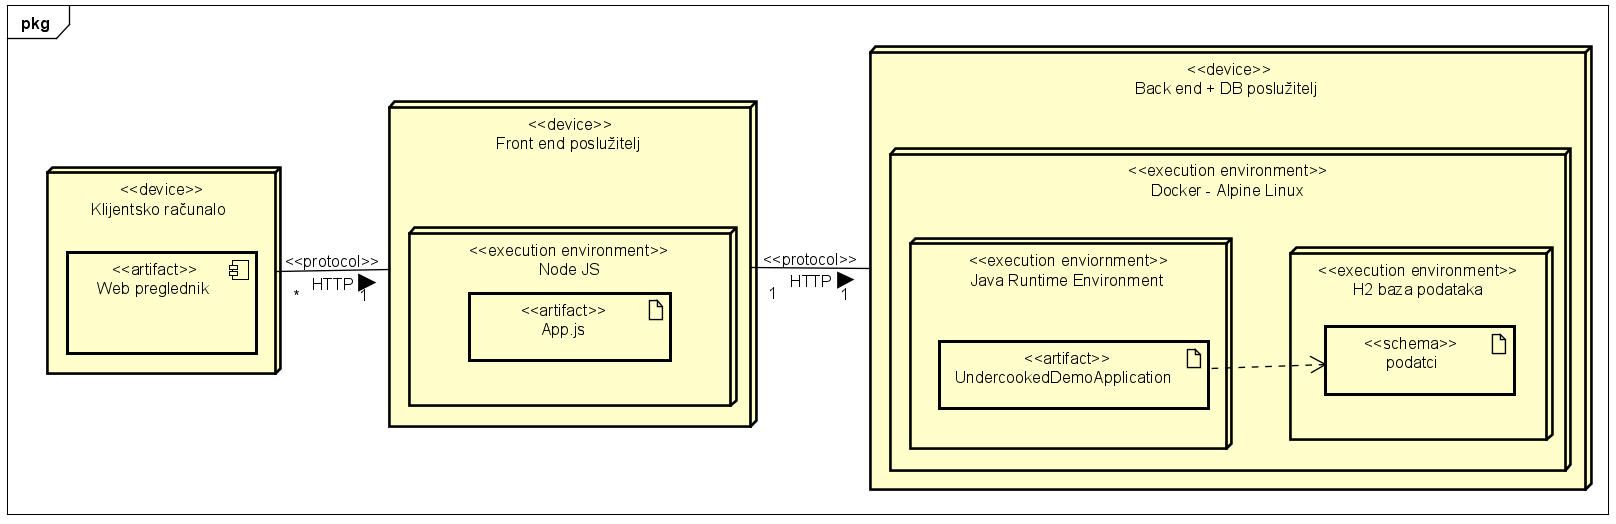
\includegraphics[scale=0.35]{slike/dijagram_razmjestaja.png} %veličina slike u odnosu na originalnu datoteku i pozicija slike
				\centering
				\caption{Dijagram razmještaja}
				\label{fig:Dijagram razmještaja}
			\end{figure}
			\eject 
		
		\section{Upute za puštanje u pogon}
		
			%\textbf{\textit{dio 2. revizije}}\\
		
			 %\textit{U ovom poglavlju potrebno je dati upute za puštanje u pogon (engl. deployment) ostvarene aplikacije. Na primjer, za web aplikacije, opisati postupak kojim se od izvornog kôda dolazi do potpuno postavljene baze podataka i poslužitelja koji odgovara na upite korisnika. Za mobilnu aplikaciju, postupak kojim se aplikacija izgradi, te postavi na neku od trgovina. Za stolnu (engl. desktop) aplikaciju, postupak kojim se aplikacija instalira na računalo. Ukoliko mobilne i stolne aplikacije komuniciraju s poslužiteljem i/ili bazom podataka, opisati i postupak njihovog postavljanja. Pri izradi uputa preporučuje se \textbf{naglasiti korake instalacije uporabom natuknica} te koristiti što je više moguće \textbf{slike ekrana} (engl. screenshots) kako bi upute bile jasne i jednostavne za slijediti.}
			
			
			 %\textit{Dovršenu aplikaciju potrebno je pokrenuti na javno dostupnom poslužitelju. Studentima se preporuča korištenje neke od sljedećih besplatnih usluga: \href{https://aws.amazon.com/}{Amazon AWS}, %\href{https://azure.microsoft.com/en-us/}{Microsoft Azure} ili \href{https://www.heroku.com/}{Heroku}. Mobilne aplikacije trebaju biti objavljene na F-Droid, Google Play ili Amazon App trgovini.}
			\subsection{Instalacija potrebne programske potpore}
			Kako bi se aplikacija ispravno pokrenula potrebno je preuzeti sljedeće programske pakete:
			\begin{itemize}
				\item \href{https://nodejs.org}{\textit{NodeJS}\footnote{https://nodejs.org}} i \href{https://www.npmjs.com}{\textit{npm}\footnote{https://www.npmjs.com}} za pokretanje front-enda
				\item \href{https://www.oracle.com/java/technologies/downloads/\#java17}{\textit{Java development kit} (Verzija 17)\footnote{https://www.oracle.com/java/technologies/downloads/\#java17}} i \href{https://maven.apache.org}{\textit{Maven}\footnote{https://maven.apache.org}} za back-end i bazu podataka.
			\end{itemize}
			\begin{figure}[H]
				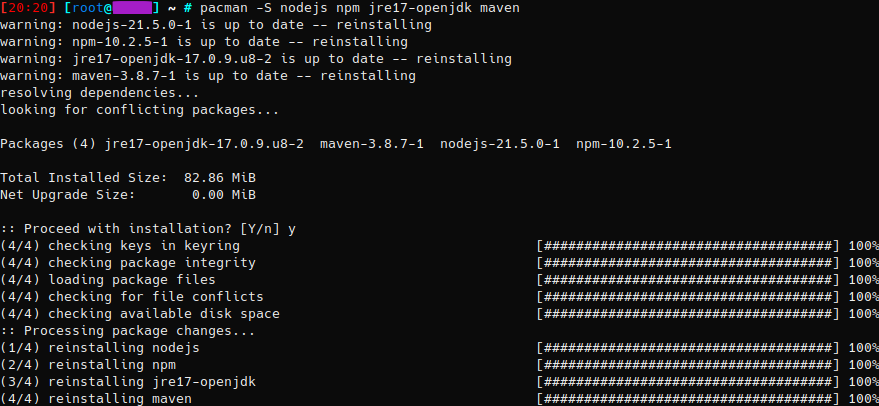
\includegraphics[scale=0.7]{slike/instalacija_1.png} %veličina slike u odnosu na originalnu datoteku i pozicija slike
				\centering
				\caption{Instalacija potrebne programske potpore na Linuxu}
				\label{fig:Instalacija potrebne programske potpore na Linuxu}
			\end{figure}
			Alternativno, back-end i baza podataka mogu se jednostavnije pokrenuti u \href{https://www.docker.com}{\textit{Docker}\footnote{https://www.docker.com}} kontejneru.
			
			Nakon instalacije navedenih programa, potrebno je klonirati repozitorij aplikacije na proizvoljnu lokaciju ili ga preuzeti kao arhivu i raspakirati.
			\begin{figure}[H]
				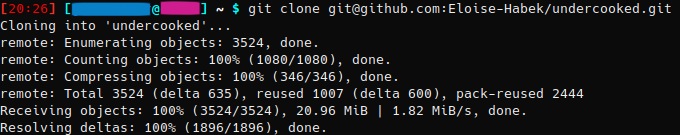
\includegraphics[scale=0.8]{slike/instalacija_2.png} %veličina slike u odnosu na originalnu datoteku i pozicija slike
				\centering
				\caption{Kloniranje repozitorija}
				\label{fig:Kloniranje repozitorija}
			\end{figure}
			\subsection{Pokretanje front-enda}
			Kako bi se pokrenuo front-end aplikacije, potrebno je pozicionirati se u direktorij \textit{IzvorniKod/undercooked-frontend} i pokrenuti \textit{npm install} kako bi se instalirale potrebne biblioteke.
			\begin{figure}[H]
				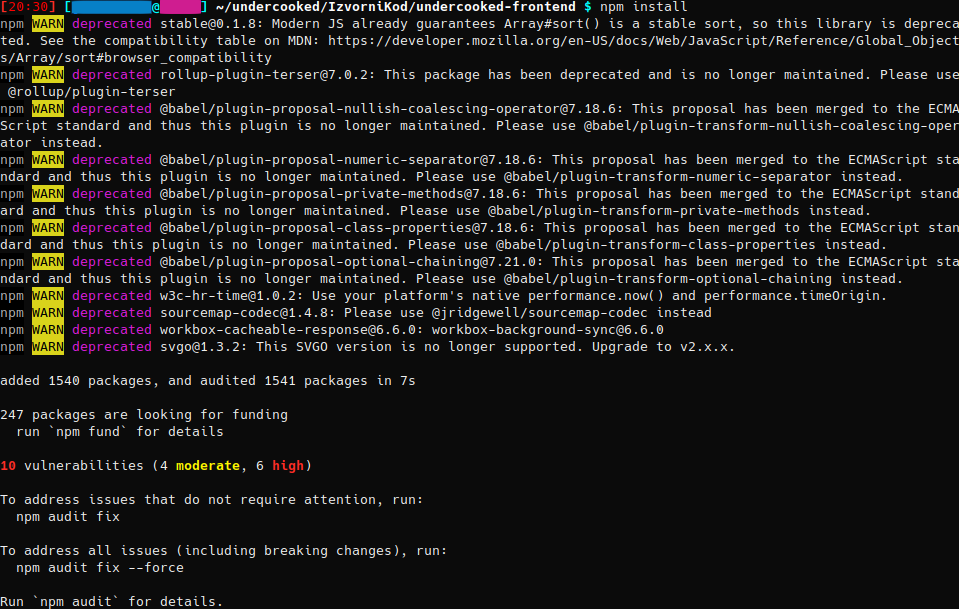
\includegraphics[scale=0.6]{slike/instalacija_3.png} %veličina slike u odnosu na originalnu datoteku i pozicija slike
				\centering
				\caption{Instalacija NodeJS biblioteka}
				\label{fig:Instalacija NodeJS biblioteka}
			\end{figure}
			Nakon toga, front-end aplikacije može se pokrenuti s \textit{npm start}. \textit{React} front-end pokreće se na vratima 3000, osim ako nije postavljena varijabla okruženja PORT.
			\begin{figure}[H]
				
\includegraphics[scale=0.7]{slike/instalacija_4.png} %veličina slike u odnosu na originalnu datoteku i pozicija slike
				\centering
				\caption{Pokretanje front-enda}
				\label{fig:Pokretanje front-enda}
			\end{figure}
			\subsection{Pokretanje back-enda i baze podataka}
			Kako bi se pokrenuli back-end aplikacije i baza podataka, potrebno je pozicionirati se u direktorij \textit{IzvorniKod/Undercooked-Demo} i pokrenuti \textit{mvn install} čime se instalira sve što je potrebno za pokretanje back-enda i baze podataka te se gradi sama aplikacija.
			\begin{figure}[H]
				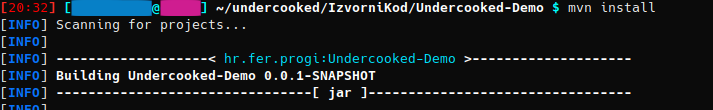
\includegraphics[scale=0.8]{slike/instalacija_5.png} %veličina slike u odnosu na originalnu datoteku i pozicija slike
				\centering
				\caption{Instalacija uz pomoć Mavena}
				\label{fig:Instalacija uz pomoć Mavena}
			\end{figure}
			Ova naredba će također pokrenuti i testove, no svi ispitni slučajevi koji koriste \textit{Selenium} će pasti jer se oslanjaju na to da back-end radi, a pokreću se prije nego što se on pokrene. Testovi se mogu izvršiti naknadno, na primjer iz IDE-a. Nakon što je izgrađena, aplikacija se može pokrenuti navigiranjem u novonastali direktorij \textit{target} i izvršavanjem naredbe \textit{java -jar Undercooked-Demo-0.0.1-SNAPSHOT.jar}. Back-end aplikacije sluša na vratima 8080, a pokretanjem back-enda pokreće se i baza podataka.
			\begin{figure}[H]
				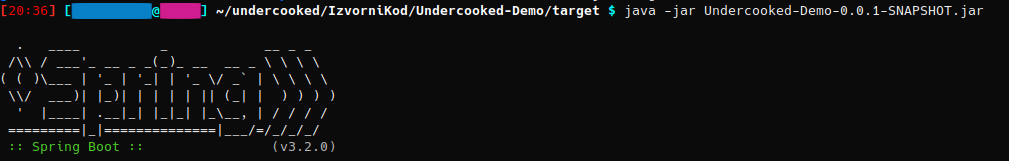
\includegraphics[scale=0.55]{slike/instalacija_6.png} %veličina slike u odnosu na originalnu datoteku i pozicija slike
				\centering
				\caption{Pokretanje back-enda i baze podataka}
				\label{fig:Pokretanje back-enda i baze podataka}
			\end{figure}
			\eject 